% !TEX encoding = UTF-8
% !TEX TS-program = pdflatex
% !TEX root = ../tesi.tex
\newpage
%**************************************************************
\chapter{Contesto Aziendale}
\label{cap:introduzione}

\section{L'azienda}
\AD{} è una start-up nata nel 2014, dall'idea di tre giovani padovani, Carlo Pasqualetto, Jacopo Pertile e Antonio Fornari, con l'intento di assistere le aziende nel miglioramento e nella digitalizzazione dei propri processi interni.\\
Inizialmente, \AD{} si rivolgeva ad un pubblico formato da piccole e medie imprese, fornendo loro consulenze di strategie aziendali, formazione del personale sugli strumenti digitali da utilizzare e piccoli software su misura.\\
Il salto di qualità avviene del 2016, quando \AD{} partecipa ad una competizione organizzata dal colosso svedese degli elettrodomestici Electrolux, per sviluppare un progetto di pianificazione intelligente della forza lavoro.

\begin{figure}[h]

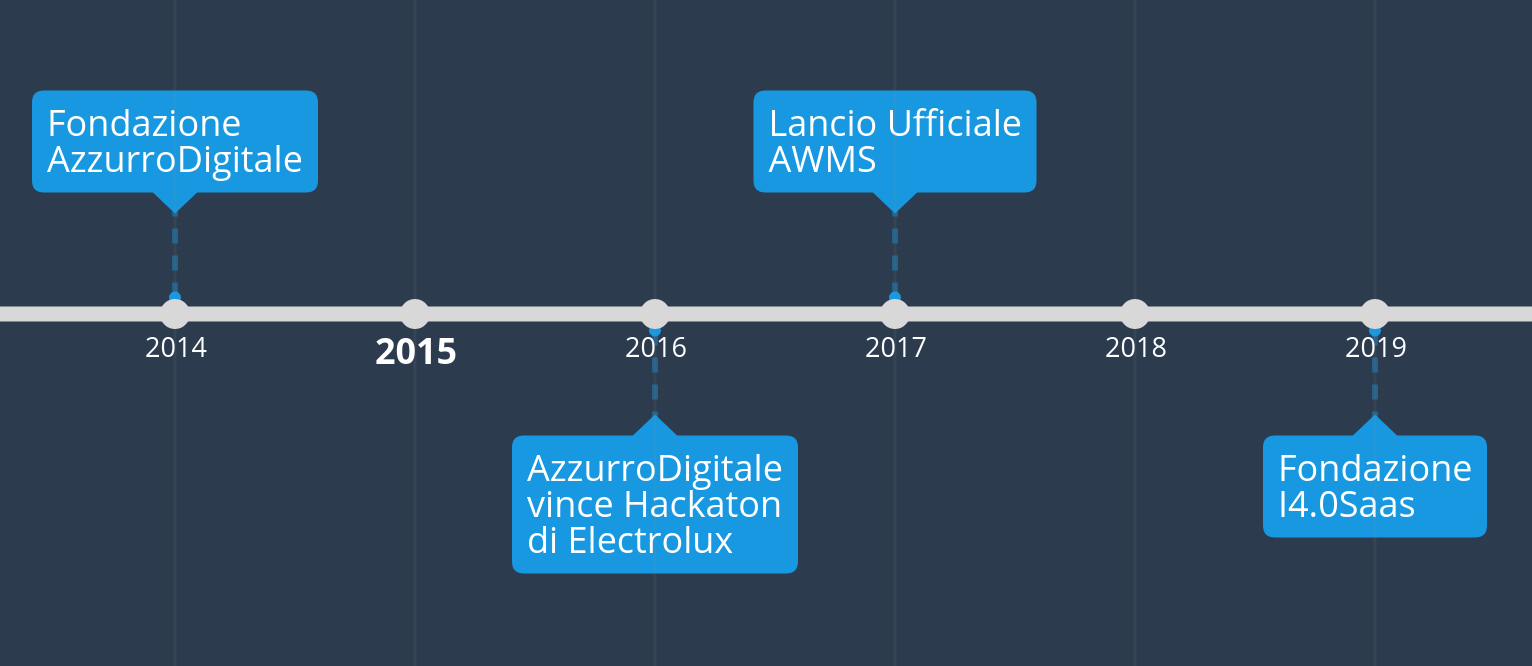
\includegraphics[width=0.8\textwidth]{AD_timeline.png}
\centering
\caption{Punti focali della storia di \AD{}.}
\end{figure}
La vittoria di questa competizione, ha portato alla nascita del progetto AWMS, prodotto di punta di \AD{}.\\
Vista la grossa richiesta di AWMS da parte di importanti aziende nazionali ed internazionali, nel 2019 i tre soci decidono di dare vita ad \textbf{I4.0Saas}, uno \textit{spin-off} di \AD{}, che a partire dal 2020 si occuperà esclusivamente della gestione e dello sviluppo del progetto AWMS.\\

\subsection{Obiettivi e valori}
%descrizione degli obiettivi (ovvero DOVE l'azienda sta puntando ad arrivare) e i valori cardine dell'azienda (Azzurrite)\\

%%%%%%%%%%%%%%%%%%%%%%%%%%%%%%%%%%%%%%%%%%%%%%%%%%%%%%%%%%%%%%%%%%%%%%%%%%%%%%%%%%%%%%%%%%%
\AD{} è una start-up in forte crescita, che ambisce ad entrare con le proprie soluzioni nelle realtà delle maggiori aziende manifatturiere mondiali.

La sua ascesa nel mondo dell'\textit{Industria 4.0} e della \textbf{\textit{digital transformation}} è frutto dei solidi principi sui quali l'azienda è fondata.\\
La filosofia aziendale di \AD{} infatti, pone in rilievo la \textbf{Persona} e le \textbf{Idee}: questo consente ad ogni dipendente di essere allo stesso livello, nonostante le differenze di mansione e di anzianità lavorativa.\\
Un altro pilastro fondante di \AD{} è il concetto di \textbf{Squadra}: non è raro infatti, che vengano effettuate delle sessioni di \textit{brainstorming} tra tutto il personale per trovare idee innovative o soluzioni a problematiche riscontrate nei vari progetti.\\

%%%%%%%%%%%%%%%%%%%%%%%%%%%%%%%%%%%%%%%%%%%%%%%%%%%%%%%%%%%%%%%%%%%%%%%%%%%%%%%%%%%%%%%%%%%



\subsection{Modello di business}
%descrizione del modello di business (AzzurroDigitale: strategies and ventures)\\
Il modello di business principale di \AD{} si orienta fondamentalmente sulla \textit{digital transformation} delle aziende.
In questo frangente, nello specifico, \AD{} opera in due settori:
\begin{itemize}
\item \textbf{Gestione della forza lavoro:} ovvero la pianificazione ottimale delle risorse umane all'interno di un reparto produttivo;
\item \textbf{Digitalizzazione dei processi aziendali:} ovvero la trasposizione in maniera automatica e digitale di tutte le attività di un processo che in precedenza venivano effettuate manualmente o in maniera non automatizzata, così da migliorare l'efficienza del processo stesso. 
\end{itemize}
\begin{figure}[h]
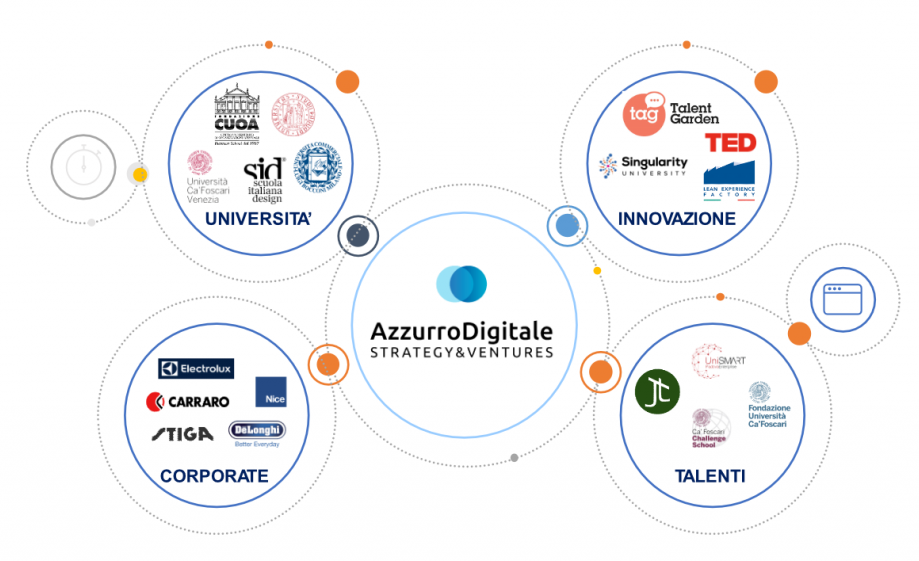
\includegraphics[width=0.9\textwidth]{AD-network.png}
\centering
\caption{Innovation Network di AzzurroDigitale.} 
\source{\href{https://www.azzurrodigitale.com/}{Azzurrodigitale.com}}
\label{fig:innovation-network}
\end{figure}
Lavorando a stretto contatto con l'ambiente universitario, \AD{} organizza anche laboratori didattici interattivi, nei quali gli studenti si troveranno ad affrontare alcune delle sfide del mondo lavorativo, proposte da aziende partner.

\subsection{Prodotti e \textit{spin-off}}
%- panoramica sulle tipologie di prodotti realizzate (trasformazione digitale delle aziende)\\
%- spin-off: I4.0Saas\\
I prodotti realizzati da \AD{} riguardano, come accennato, il settore manifatturiero e la gestione della forza lavoro.
Sin dalla sua nascita infatti, \AD{} ha offerto ai propri clienti, software su misura per il monitoraggio e per il miglioramento dei processi legati al reparto di produzione.\\
Tra questi, è bene citare \textit{Digital Cockpit}: una \textit{web-app} sviluppata in collaborazione con Safilo Group, azienda tra i leader mondiali nella produzione di occhiali.\\
Si tratta di un'applicazione che monitora i macchinari del reparto produzione e ne registra tutti i parametri di lavoro, fornendo così un cruscotto informativo completo sull'efficienza giornaliera del macchinario, oltre alle tempistiche di lavoro, ai dettagli del prodotto in fase di lavorazione e ai tempi morti del macchinario stesso.\\
Aumentando il numero di clienti, \AD{} ha cominciato a sviluppare anche software non legati al singolo cliente, rimanendo sempre nell'ambito della \textit{digital transformation}:
\begin{itemize}
\item \textbf{AWMS:} \textit{Advanced Workforce Management System} è una soluzione software che, tramite algoritmi di \textit{machine learning}, si occupa di pianificare in maniera ottimale la forza lavoro all'interno di uno stabilimento produttivo, tenendo conto di assenze inaspettate, livello di esperienza dell'operatore in una determinata mansione e certificazioni possedute da quest'ultimo. \\
Si tratta del prodotto di punta di \AD{} ed attualmente figurano tra i suoi utilizzatori, aziende rinomate come Electrolux, Safilo Group, Zoppas Industries, Stiga e Ferrari;
\item \textbf{DigitalSnapshots:} Software sviluppato in collaborazione con Electrolux, ha lo scopo di monitorare lo stato di avanzamento dei progetti all'interno dei vari stabilimenti, fornendo così una panoramica sulle risorse impegnate e/o mancanti nei singoli progetti, la percentuale di avanzamento del progetto stesso, ed il peso in termini di importanza che quel progetto ha all'interno dello stabilimento.
\end{itemize}

\subsubsection*{\textit{Spin-off}}
Come accennato ad inizio capitolo, nel corso del 2019 è nata \textbf{I4.0Saas}, ovvero un distaccamento di \AD{} che a partire dal 2020 andrà ad occuparsi della vendita, della gestione e dello sviluppo del software AWMS.

\section{Organizzazione interna}
%Organizzazione aziendale: team sviluppo e team consulenze. Descrizione dettagliata di entrambi
Come descritto in precedenza, \AD{} crede fortemente nel capitale umano e nello spirito di squadra. Per questo motivo, all'interno di essa non esiste una netta gerarchia del personale: ogni dipendente è considerato alla pari, ed ogni idea o proposta viene discussa e valutata senza pregiudizio. \\
Tuttavia, il personale può essere suddiviso in base alle competenze e alla propria mansione all'interno dell'azienda. Possiamo quindi trovare i seguenti reparti:
\begin{itemize}
\item \textbf{\textit{Development}}\\
Questo reparto ha il compito di sviluppare il prodotto, definendo ed implementando tutte le caratteristiche accordate con il cliente, sia a livello logico (\textit{back-end}) che a livello visuale (\textit{front-end}). Fa parte di questo reparto anche la figura del designer, che ha il compito di definire l'interfaccia utente alla quale poi gli sviluppatori dovranno far riferimento;  
\item \textbf{\textit{Consulting}}\\
Questo è un reparto chiave per il modello di business di \AD{}. E\'{} formato da consulenti che hanno lo scopo di analizzare i processi aziendali dei clienti, individuare le inefficienze e proporre delle soluzioni o delle strategie affinché venga massimizzata l'efficienza dello stabilimento. Inoltre, svolgono il ruolo di analista funzionale, che si pone tra il cliente e il team di sviluppo, così da facilitare l'implementazione delle funzionalità richieste;
\item \textbf{\textit{Human Resources} e \textit{Formation}}\\
I membri del reparto delle risorse umane hanno un duplice compito in azienda: in primis, si occupano di contattare, valutare ed eventualmente inserire nuovi innesti nei vari reparti. Inoltre, si dedicano alla preparazione di eventi sulla formazione del personale;
\item \textbf{Amministrazione, Finanza e Controllo}\\
Questo reparto si occupa della parte economica dell'azienda, gestendo il personale, le spese e i ricavi, verificando inoltre il corretto andamento di tutti i reparti.
\end{itemize}

\section{Processi Aziendali}
%metodologia scrum applicata sia nel team sviluppo, sia nel team consulenze
Un'adeguata organizzazione interna è fondamentale per raggiungere gli obiettivi e per offrire ai clienti dei servizi adeguati. Pertanto è richiesta la coordinazione tra tutti i reparti, in modo da raggiungere lo scopo aziendale comune.

\subsubsection*{Comunicazione}
Le comunicazioni interne all'azienda e con i clienti, avvengono prevalentemente tramite e-mail aziendale, così da rendere i contenuti più tracciabili.\\
Per le comunicazioni più informali ed immediate, invece, si utilizzano software di messaggistica istantanea, quali \textit{Slack}, utilizzato soprattutto nel reparto di sviluppo in quanto permette la creazione di canali di comunicazione specifici per ogni progetto, e \textit{Telegram}, per le comunicazioni generali.

\subsubsection*{Gestione di progetto}
Per la gestione del progetto, l'azienda si avvale di molteplici strumenti, a seconda delle diverse fasi ed esigenze:
\begin{itemize}

\item \textbf{Microsoft Office:} Per tutta la documentazione, dalle offerte al tracciamento dei requisiti, passando per la manualistica, viene utilizzata la suite Office di Microsoft;

\item \textbf{Asana:} Questa applicazione viene utilizzata dal \textit{Project Manager} per l'amministrazione della pianificazione. Essa permette infatti di coordinare le risorse, gestire i task e creare i diagrammi di Gantt, a supporto di uno specifico progetto;

\item \textbf{Time Report:} Si tratta di un software sviluppato internamente, viene utilizzato per organizzare e tenere traccia delle ore svolte dai singoli dipendenti per ogni commessa a loro assegnata. Grazie alla sua integrazione con un \textit{bot} di \textit{Telegram}, viene utilizzato anche per la segnalazione rapida delle assenze o dei giorni di ferie;

\item \textbf{Google Calendar:} Questo servizio viene utilizzato per indicare gli impegni di ogni dipendente, in modo da avere una panoramica sulla disponibilità di risorse umane. In aggiunta, viene utilizzato anche per la prenotazione della sala riunioni.
\end{itemize}

\subsubsection*{Sviluppo}
La metodologia di sviluppo adottata nell'azienda riguarda il \textbf{modello Agile} i cui principi sono riassunti nel Manifesto Agile\footnote{\textit{Manifesto Agile.} URL: \href{http://agilemanifesto.org/iso/it/}{http://agilemanifesto.org/iso/it/}}. 
Nello specifico, viene seguito il \textit{framework} Scrum, sintetizzato in figura \ref{fig:scrum}.
Questa metodologia prevede di suddividere il progetto in più fasi, dette Sprint. L'obiettivo di ogni Sprint, chiamato Sprint Goal, è quello di portare un prodotto non finito, ma potenzialmente completo e funzionante, secondo gli avanzamento pianificati per il singolo ciclo. Il susseguirsi di questi cicli di durata fissa, nel mio caso di due settimane, porta incrementi al prodotto fino a che questo non soddisfi tutti i requisiti delineati.
Il \textit{framework} Scrum è caratterizzato da una serie di attività prestabilite:
\begin{itemize}
\item \textbf{Product Backlog:} ovvero una lista di tutte le attività, funzionalità e requisiti del prodotto;
\item \textbf{Sprint Planning:} si tratta di una riunione svolta all'inizio di ogni Sprint, ed ha lo scopo di definire gli obiettivi da raggiungere (\textit{Sprint Goal}) e di pianificare le modalità di come portarli a termine (\textit{Sprint Backlog});
\item \textbf{Daily Scrum:} riunione giornaliera in cui il team di sviluppo si aggiorna su cosa è stato fatto il giorno precedente, cosa verrà fatto nelle successive ore lavorative ed eventuali difficoltà affrontate. Lo scopo principale del Daily Scrum è semplificare la collaborazione e l'allineamento del lavoro, e risolvere eventuali problemi di avanzamento in maniera tempestiva;
\item \textbf{Sprint Review:} Alla fine dello Sprint si tiene l'incontro di Sprint Review per ispezionare l'incremento e adattare, se necessario, il Product Backlog. Durante la riunione di Sprint Review il Team di Sviluppo e gli \textit{stakeholder} collaborano su ciò che è stato fatto durante lo Sprint. In conformità a questo e dei cambiamenti al Product Backlog fatti durante lo Sprint, i partecipanti collaborano sulle prossime cose che potrebbero esser fatte. Si tratta di un incontro informale e la presentazione dell'incremento apportato al prodotto ha lo scopo di suscitare commenti e promuovere la collaborazione;
\item \textbf{Sprint Retrospective:} La Sprint Retrospective è l'occasione per il Team Scrum per ispezionare se stesso e creare un piano di miglioramento da attuare durante il prossimo Sprint.
\end{itemize}
\begin{figure}[h]
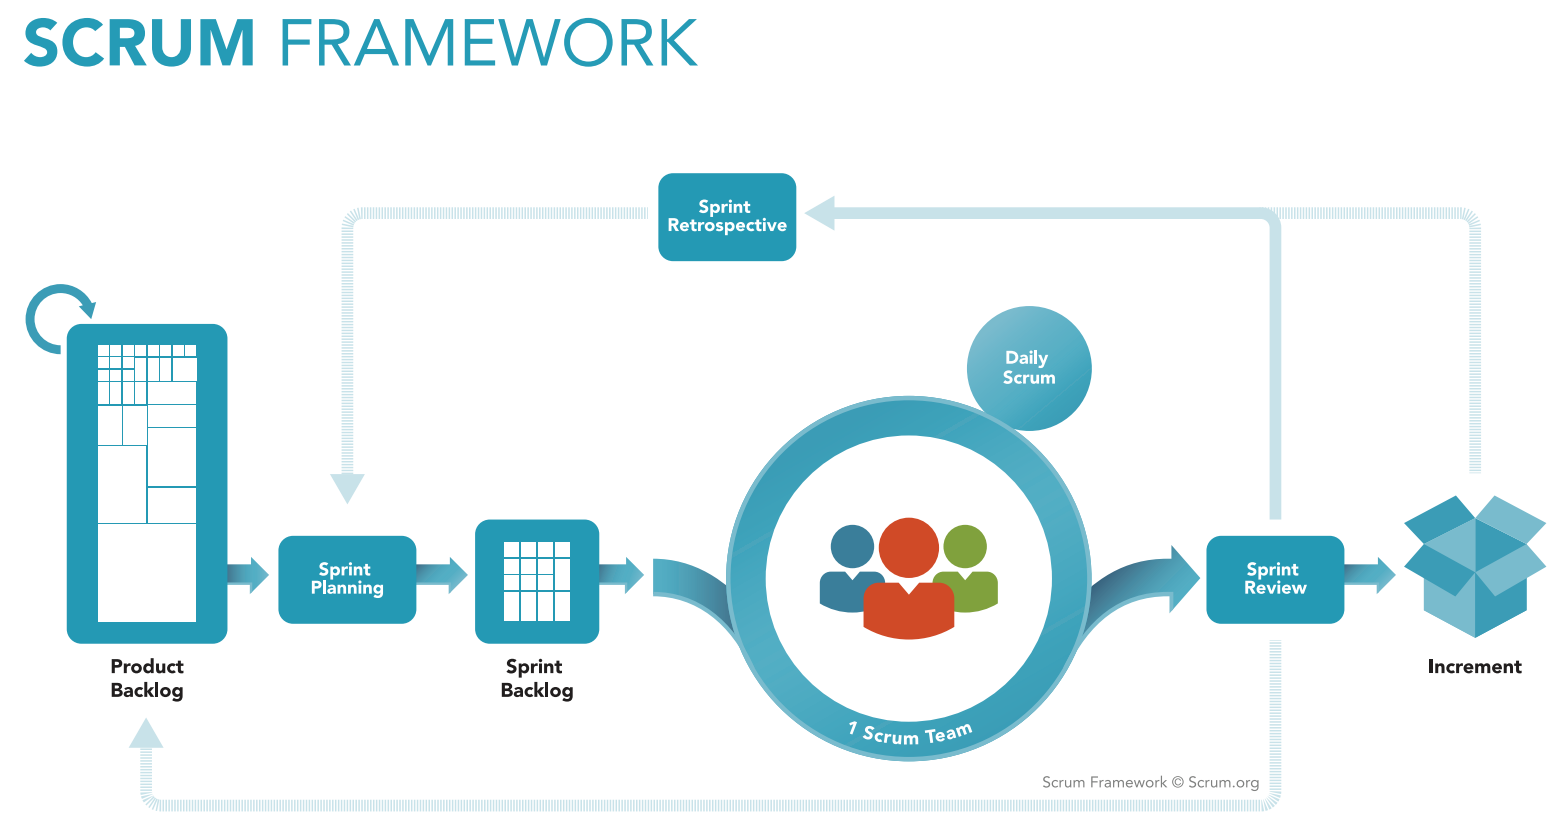
\includegraphics[width=\textwidth]{agile-scrum.png}
\centering
\caption{Rappresentazione del \textit{framework} Scrum.}
\source{\href{https://www.scrum.org/}{Scrum.org}}
\label{fig:scrum}
\end{figure}
\AD{} ha deciso di adottare la metodologia agile per lo sviluppo software in quanto permette all'azienda di essere molto elastica rispetto ad eventuali cambiamenti dei requisiti iniziali, oltre che a permettere il \textit{deploy} di un prodotto testabile al termine di ogni Sprint, così da avere un \textit{feedback} sul prodotto nel minor tempo possibile ed agire tempestivamente su modifiche o correzioni di errori.  

\subsubsection*{\textit{Consulting}}
A differenza del reparto di sviluppo, il reparto di \textit{consulting} ha adottato un approccio lavorativo originale, studiato e realizzato in collaborazione con il dipartimento di Ingegneria Gestionale dell’Università di Padova, chiamato \textbf{\textit{"The digitalization factory loop"}}.\\
\`E possibile riassumere questo approccio in tre semplici frasi, ognuna delle quali corrisponde ad una fase del processo, \textit{“Make it Clear, Make it Tangible, Make it Real”}.
Questo approccio dunque, consiste nello scomporre il processo in 3 fasi distinte e ripeterle fino al raggiungimento dell'obiettivo:
\begin{itemize}
\item \textbf{\textit{Make it clear}:} in questa fase si definiscono degli obiettivi digitali prioritari cercando di comprendere come la tecnologia può essere utilizzata per il successo aziendale e in che modo è bene indirizzare gli investimenti;
\item \textbf{\textit{Make it Tangible}:} dagli obiettivi digitali si passa ai progetti digitali, così da definire in modo tangibile la strategia digitale. In questo step dei team operativi composti da impiegati verranno creati per generare la strategia;
\item \textbf{\textit{Make it Real}:} in questa fase i progetti vengono concretamente realizzati attraverso un’implementazione day-by-day e la coordinazione dei team di lavoro con specifiche metodologie di project management.
\end{itemize}

\begin{figure}[h]

\includegraphics[width=\textwidth]{makeitreal.png}
\centering
\caption{Rappresentazione del \textit{digitalization factory loop}.} 
\source{\href{https://www.azzurrodigitale.com/}{Azzurrodigitale.com}}
\label{fig:make-it-real}
\end{figure}
